\section{Résultats}
Afin d'analyser les performances de la méthode proposée par \cite{bib_gicp}, nous avons tout d'abord chercher à étudier l'influence du critère $d_{max}$ appliquer lors de l'appariement des points, la robustesse de l'algorithme face à des changement de poses différents et la différence de résultats entre le Standard ICP obtenu avec la formule analytique et le Standard ICP obtenu avec le modèle probabilistique présenté dans l'article. (en posant $C_{i}^B=Id$ et $C_{i}^A=0$).\\

Etant donné que GICP utilise l'information des surfaces de chacun des nuages de points, l'algorithme présente donc théoriquement une meilleure robustesse à la différence d'échantillonnage entre les deux nuages de points. Ainsi, l'ensemble des tests seront réalisés à la fois sur une paire de scans synthétiques présentée dans la figure \ref{fig_nuage_bunny} et une paire de scans réelles acquise par l'université de Hannovre présentée dans la figure \ref{fig_nuage_recalage} . On dispose pour les scans réels de l'estimation de leur poses, i.e une matrice de transformation $T^*$, afin de s'en servir de vérité terrain. Enfin, pour générer la paire de scans synthétiques, une transformation connue $T^{*}$ est appliquée sur le nuage de points synthétiques puis la position des points du nuage transformé est modifié par un bruit gaussien.\\

La transformation initiale $\mathbf{T}_0$ est définie comme la transformation exacte $\mathbf{T}^*$ auquel on ajoute une erreur entre $\pm1.5m$ et $\pm15^{\circ}$ selon tous les axes. Afin d'évaluer les performances, on mesure l'erreur de position moyenne $||B - \mathbf{T}(A)||_2$ (expliquer comme on gère lorsque les nuages ne sont pas échantillonnés pareil dans la prochaine partie (erreur plus élevée, NN plus compliqué). 
\subsection{Etude de l'influence de $d_{max}$}
\label{part:influencedmax}
%Explication de d_max
La mise en correspondance des points des deux nuages est une étape cruciale de l'algorithme ICP. La solution la plus répandue consiste à apparier les points par recherche du plus proche voisin. Cependant les nuages ne se recoupent pas complètement ainsi certains points d'un nuage ne corresponde à aucun point de l'autre nuage (occlusion, recouvrement partiel). Pour prendre cela en compte, une solution est de retirer les points appariés dont la distance est supérieure à un seuil $d_{max}$.\\

%Etude théorique : +dmax petit, +précis mais moins de chance de convergence et inversement
En général, le choix de $d_{max}$ est un compromis entre la précision de l'algorithme et sa portée de convergence. En effet, une valeur faible de $d_{max}$ entraîne un faible nombre de points appariés rendant la convergence de l'algorithme plus difficile. Au contraire, une valeur plus élevée de $d_{max}$ peut causer des appariements inexactes et ainsi éloigner l'estimation de la transformation de sa valeur exacte. 

%Présentation des résultats
Afin d'évaluer l'influence de $d_{max}$ sur la performance de la méthode proposée, l'erreur de position moyenne a été mesuré sur les résultats obtenus par l'algorithme standard de l'ICP et par GICP pour différentes valeurs de $d_{max}$ sur les jeux de donnée  synthétique et réel.\\


\begin{figure}[!h]
   \centering
   \begin{subfigure}[t]{.5\linewidth}
     \centering
     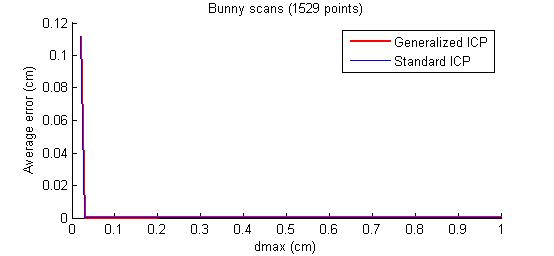
\includegraphics[scale=0.4]{Images/Resultats/bunny_evol_error_dmax.jpg}
     \caption{Données synthétiques}
     \label{fig:err_dmax_synthe}
   \end{subfigure}%
   ~
   \begin{subfigure}[t]{.5\linewidth}
     \centering
     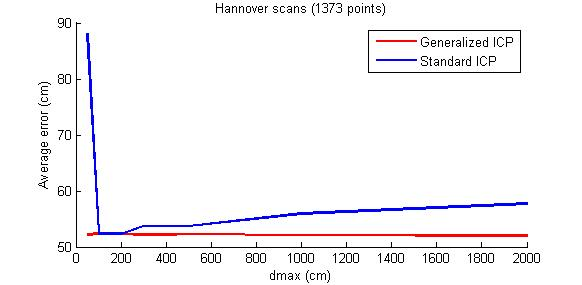
\includegraphics[scale=0.4]{Images/Resultats/hannover_evol_error_dmax.jpg}
     \caption{Données réelles}
     \label{fig:err_dmax_reelle}
   \end{subfigure}
   
   \caption{Evolution de l'erreur de position moyenne en fonction de la valeur du seuil $d_{max}$.}
   \label{fig:err_dmax}
\end{figure}



\begin{figure}[!h]
   \centering
   \begin{subfigure}[t]{.5\linewidth}
     \centering
     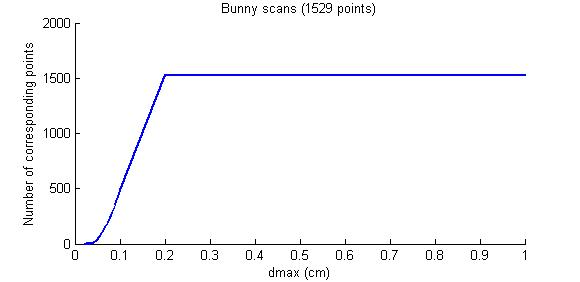
\includegraphics[scale=0.4]{Images/Resultats/bunny_size_subset_dmax.jpg}
     \caption{Données synthétiques}
     \label{fig:subset_dmax_synthe}
   \end{subfigure}%
   ~
   \begin{subfigure}[t]{.5\linewidth}
     \centering
     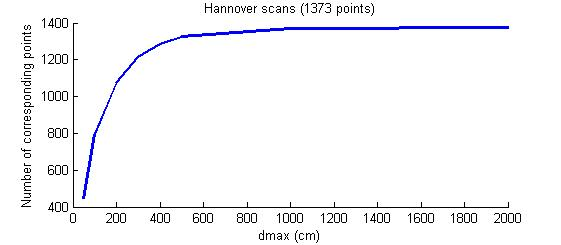
\includegraphics[scale=0.4]{Images/Resultats/hannover_size_subset_dmax.jpg}
     \caption{Données réelles}
     \label{fig:subset_dmax_reelle}
   \end{subfigure}
   
   \caption{Evolution du nombre de points appariés lors de la première itération de l'algorithme en fonction de la valeur du seuil $d_{max}$.}
   \label{fig:subset_dmax}
\end{figure}

Tout d'abord, on peut constater que pour une valeur trop faible de $d_{max}$, l'algorithme ne converge ni sur les données synthétiques, ni sur les données réelles car l'ensemble des points appariés est trop faible pour permettre à l'algorithme de converger (comme le montre le nombre de points appariés lors de la première itération de l'algorithme pour une valeur faible de $d_{max}$ sur la figure \ref{fig:subset_dmax}).\\

L'absence d'occlusion et l'échantillonnage identique entre les deux nuages synthétiques entrainent une influence nulle de $d_{max}$ sur la performance du recalage sur les données synthétiques. En effet, les nuages de point parviennent toujours à se recaler.\\

Au contraire, sur les données réelles, on peut voir que l'erreur moyenne se dégrade pour l'ICP standard lorsque $d_{max}$ dépasse une certaine valeur, $d_{max}=200$. Tandis que l'influence sur GICP reste très faible. En effet, de nombreux appariements sont inexactes lorsque la valeur de $d_{max}$ est élevée ce qui à pour conséquence d'éloigner le résultat de la solution exacte.\\

Cependant, pour GICP, ces appariements erronés contribue très peu à la fonction de coût car ils ont peu de chance d'être coplanaire (voir la figure \ref{fig_cov}). Ainsi, comme le montre la figure \ref{fig:err_dmax_reelle}, l'erreur moyenne est stable lorsque la valeur de $d_{max}$ augmente pour GICP tandis qu'elle se dégrade pour l'ICP standard.\\

\begin{figure}[!h]
   \centering
   \begin{subfigure}[t]{.5\linewidth}
     \centering
     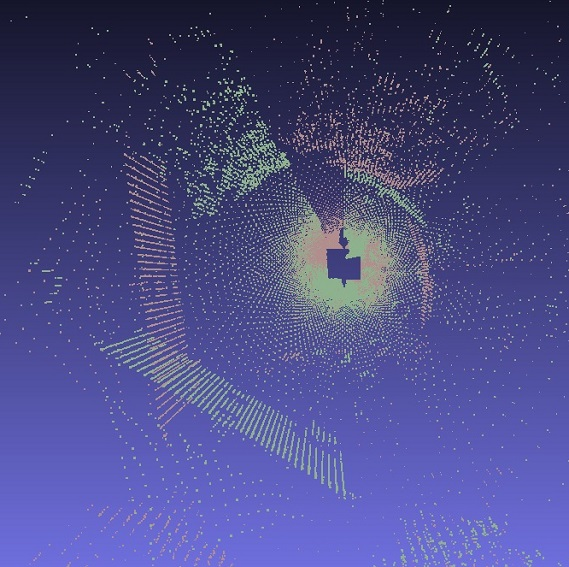
\includegraphics[scale=0.5]{Images/Resultats/hannover_meshlab_before_transformation.jpg}
     \caption{Nuages avant recalage}
   \end{subfigure}%
   ~
   \begin{subfigure}[t]{.5\linewidth}
     \centering
     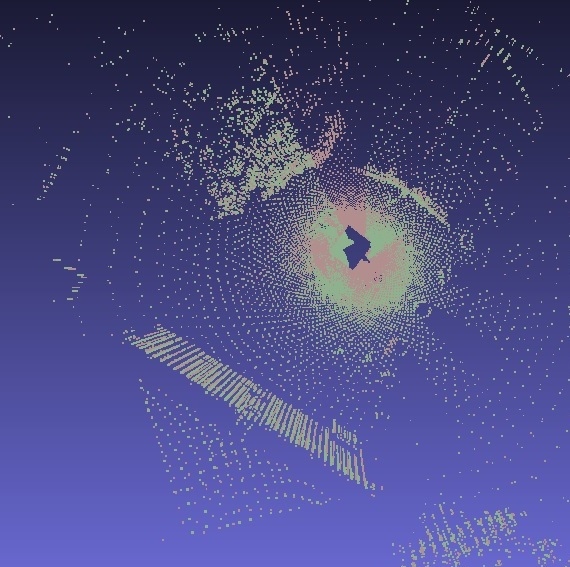
\includegraphics[scale=0.5]{Images/Resultats/hannover_meshlab_after_transformation.jpg}
     \caption{Nuages après recalage}
   \end{subfigure}
   
   \caption{A REMPLIR.}
   \label{fig:meshlab}
\end{figure}

De plus on peut aussi observer que l'erreur moyenne obtenue par GICP est toujours inférieure ou égale à celle obtenue par ICP standard. Mettant ainsi en évidence la meilleure performance de GICP par rapport à l'ICP Standard.\\

\begin{figure}[!h]
     \centering
     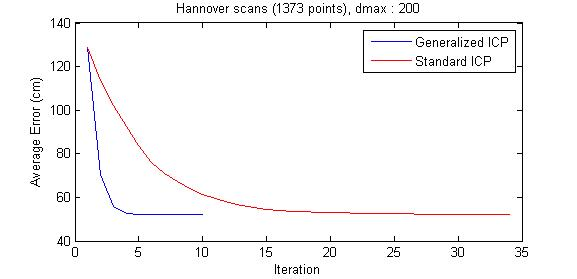
\includegraphics[scale=0.4]{Images/Resultats/hannover_dmax200_diffconvergence.jpg}
     \caption{Comparaison de la vitesse de convergence sur les données réelles pour $d_{max}=200$ entre GICP et ICP standard.}
	\label{fig:GICP_convergence}
\end{figure}

Enfin, comme le montre la figure \ref{fig:GICP_convergence}, on constate que GICP converge beaucoup plus rapidement que l'ICP Standard. (ajouter un commentaire sur le temps d'exécution GICP<<sICP car converge plus rapidement).
   
\subsection{Etude de l'influence de l'offset}

La méthode de comparaison qu'applique Segal et al. utilise toujours une transformation initiale $\mathbf{T}_0$ qui est définie comme la transformation exacte $\mathbf{T}^*$ auquelle est ajoutée une erreur entre $\pm1.5m$ et $\pm15^{\circ}$ selon tous les axes. 

L'idée ici est de comparer GICP et l'ICP standard pour des valeurs de $T_0$ beaucoup plus éloignées de $T^*$ afin d'étudier leurs robustesses face à la transformation initiale $T_0$.

Pour cela, nous avons fixé la matrice $\mathbf{T}_0=\mathbf{T}^*+\epsilon $ où $\epsilon$ est un terme d'erreur constant compris entre $\pm1.5m$ et $\pm15^{\circ}$ selon tous les axes puis nous avons fait varier l'erreur de la rotation $\theta$ autour de l'axe des $x$ entre $[-20^{\circ} -65^{\circ}]$.

\begin{figure}[!h]
   \centering
   \begin{subfigure}[t]{.5\linewidth}
     \centering
     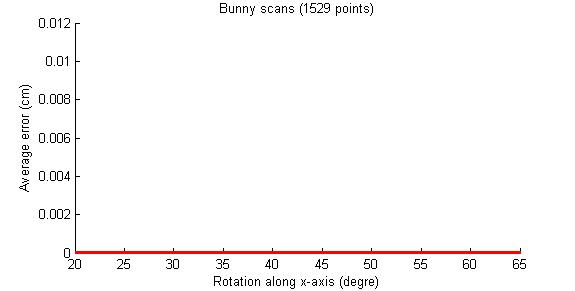
\includegraphics[scale=0.4]{Images/Resultats/bunny_offset_evol-error_sicp.jpg}
     \caption{Standard ICP}
   \end{subfigure}%
   ~
   \begin{subfigure}[t]{.5\linewidth}
     \centering
     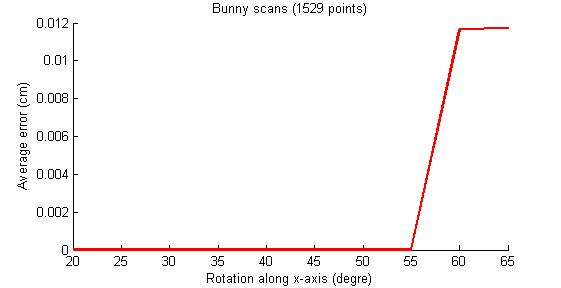
\includegraphics[scale=0.4]{Images/Resultats/bunny_offset_evol-error_gicp.jpg}
     \caption{Generalized ICP}
   \end{subfigure}
   
   \caption{Evolution de l'erreur de position moyenne en fonction de la rotation $\theta$ selon l'axe des $x$ de $\mathbf{T}_0$ sur des données synthétiques.}
   \label{fig:offset}
\end{figure}


La figure \ref{fig:offset} montre l'évolution de l'erreur moyenne de position obtenue par GICP et ICP standard en fonction de la valeur de l'angle $\theta$. On constate qu'à partir d'une certaine valeur ($\theta = -60^{\circ}$), GICP ne converge plus. Au contraire, l'ICP standard continue à converger quelque soit la valeur de $\theta$.

Ainsi, la robustesse de la méthode Generalized ICP à l'offset initial $\mathbf{T}_0$ est moins bonne que pour l'ICP standard. Il est donc important d'avoir une transformation initiale $\mathbf{T}_0$ pas trop éloignée de la transformation exacte $\mathbf{T}^*$.

\subsection{Standard ICP par solution analytique}

Comme présenté dans la partie \ref{part:impl_gicp}, le modèle probabiliste introduit par Segal permet d'implémenter différentes variantes de l'ICP en modifiant judicieusement les matrices de covariance $C_{i}^A$ et $C_{i}^B$. Ainsi, il est intéressant de comparer les résultats obtenus avec la version de l'ICP standard modélisé dans le framework GICP et les résultats obtenus avec la formule analytique de l'ICP standard. \\

Pour cela, nous avons testé l'ICP standard par formule analytique pour les mêmes valeurs de $d_{max}$ que dans la partie \ref{part:influencedmax}. Les résultats sont présentés dans la figure \ref{fig:closedform_ICP}. On peut constater que l'erreur moyenne de position obtenu est pratiquement identique entre les deux méthodes sur la figure \ref{fig:CFICP:err}. Ainsi le modèle probabiliste présenté permet bien de retrouver l'ICP standard en posant  $C_{i}^A = 0$ et $C_{i}^B = Id$.\\

\begin{figure}[!h]
   \centering
   \begin{subfigure}[t]{.5\linewidth}
     \centering
     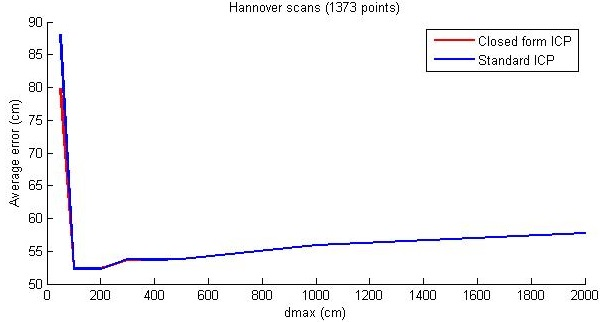
\includegraphics[scale=0.4]{Images/Resultats/hannover_diff_ICP_closed_form_dmax.jpg}
     \caption{Erreur moyenne}
     \label{fig:CFICP:err}
   \end{subfigure}%
   ~
   \begin{subfigure}[t]{.5\linewidth}
     \centering
     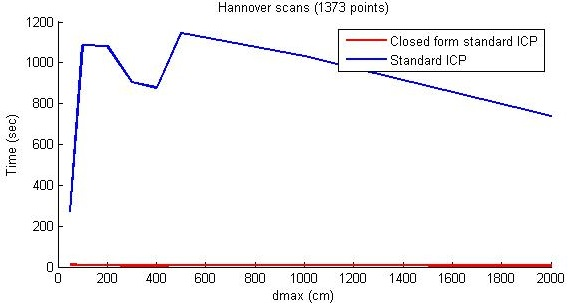
\includegraphics[scale=0.4]{Images/Resultats/hannover_diff_time_ICP_closed_form_dmax.jpg}
     \caption{Temps d'exécution}
     \label{fig:CFICP:time}
   \end{subfigure}
   
   \caption{Comparaison des résultats obtenus avec la formule analytique de l'ICP standard (en rouge) et avec le framework de GICP (en bleu).}
   \label{fig:closedform_ICP}
\end{figure}

En revanche, comme le montre la figure \ref{fig:CFICP:time}, le temps d'exécution est beaucoup plus long avec le framework GICP. Cette forte différence s'explique par l'utilisation d'une méthode de Quasi-newton pour a minimisation de l'énergie dans le framework GICP qui est très longue tandis que la minimisation est explicite dans la formule analytique de l'ICP.
